\subsection{Notation}
\begin{enumerate}\itemsep=0pt
\item[(1)] We shall use the notation $\mathit{X}^k$ to stand for the rational function $\mathit{X}^k(x) = x^k$ for $k \in \mathbb{Z}$.
\item[(2)] For $a,b \in \mathbb{Z}$, we let $[\![a,b]\!]$ be the integer interval from $a$ to $b$, $[\![a,b]\!] = [a,b] \cap \mathbb{Z}$.
\item[(3)] For $k \in \mathbb{N}$, define the space of real polynomials of degree at most $k$ as
$\mathscr{P}_{k}^\mathbb{R}$, and let
\smash{$\mathscr{P}^\mathbb{R} = \bigcup_{k\geq 0} \mathscr{P}_{k}^\mathbb{R}$} be the space of all real polynomials. Similarly, let $\mathscr{P}^\mathbb{C}_k$ be the space of polynomials with complex coefficients of degree $\leq k$ and \smash{$\mathscr{P}^\mathbb{C} = \bigcup_{k \geq 0} \mathscr{P}^\mathbb{C}_k$}.
\item[(4)] For $m$ a positive integer and $\mathbb{F}$ a field (in our case always $\mathbb{R}$ or $\mathbb{C}$), we let $\mathcal{M}_m (\mathbb{F})$ be the space of $m \times m$ matrices with entries in $\mathbb{F}$.
\item[(5)] We use the convention that $0 \in \mathbb{N}$.
\item[(6)] We denote the 1-torus as $\mathbb{T} = \{ z \in \mathbb{C} \colon |z|=1 \}$.
\item[(7)] We let $\chi_A$ be the indicator function of the set $A$, i.e., $\chi_A(x) = 1$ if $x \in A$ and $\chi_A(x) = 0$ otherwise.
\item[(8)] Let $\Gamma \subset \mathbb{C}$ be a piecewise smooth contour in $\mathbb{C}$. Then the \textit{Cauchy transform} of the measurable function $f\colon \Gamma \longrightarrow \mathbb{C}$ is defined as
\[
C_\Gamma (f) (z) = \frac{1}{2\pi {\rm i}}\int_\Gamma \frac{f(x)}{x-z} {\rm d}x,\qquad z \in \mathbb{C}\setminus \Gamma,
\]
whenever this integral exists. In our case, we will always consider sufficiently \enquote{nice} functions $f$ and contours $\Gamma$ such that the Cauchy transform is well-defined and analytic for all $z \in \mathbb{C}\setminus \Gamma$. Furthermore, we shall always consider functions with finite moments~${\int_\Gamma |x|^k |f(x)| |{\rm d}x| < +\infty}$ for all $k\geq 0$ and for which $C_\Gamma (f)(z)$ admits an asymptotic expansion in $\frac{1}{z}$ as $z \to \infty$ in the sense of Poincar\'e. More precisely, for every $K \in \mathbb{N}$, we~have
\begin{align*}
C_\Gamma (f)(z) = - \frac{1}{2\pi {\rm i}} \sum_{k=0}^K z^{-k-1} \int_\Gamma x^k f(x) {\rm d}x +\frac{z^{-K-1}}{2\pi {\rm i} } \int_\Gamma \frac{ x^{K+1} f(x)}{x-z} {\rm d}x .
\end{align*}
If $\mathrm{dist}(z,\Gamma) \geq \epsilon > 0$, we find that $\int_\Gamma \frac{ x^{K+1} f(x)}{x-z} {\rm d}x$ is bounded. However, if $f$ is analytic we may deform the contour to achieve boundedness in a full neighbourhood of (complex) infinity. This will be the case in all the Cauchy integrals that appear in this paper. The general theory of such Cauchy integrals for functions of varying degrees of decay and regularity is discussed in notes of Deift \cite{deift2019riemannhilbert} and the book of Muskhelishvilli \cite{singular}.
\end{enumerate}

\section{Riemann--Hilbert representations}\label{rhpsection}

Before proceeding, let us demonstrate that the problem we are considering is well-posed. The following proposition is of course known to experts but we include a proof to keep the presentation complete.
\begin{Proposition} The skew-symmetric bilinear form defined by \eqref{skewprod} is non-degenerate. Furthermore, the skew-norms are all positive, i.e., $h_n = \langle P_{2n}, P_{2n+1} \rangle_4 > 0$, for all $n \geq 0$.
\end{Proposition}
\begin{proof}
By one of de Bruijn's identities \cite{debruijn}, we have
\begin{equation*}
\mathrm{pf} \big( \big\langle \mathit{X}^{i-1}, \mathit{X}^{j-1} \big\rangle_4 \big)_{i,j=1}^{2n} = \frac{1}{n!} \int_{\mathbb{R}^n} \prod_{1 \leq i < j \leq n} |x_i - x_j|^4 \prod_{k=1}^n {\rm e}^{-2V(x_k)} {\rm d} x_1 \cdots {\rm d}x_n > 0,
\end{equation*}
where $\mathrm{pf}$ is the Pfaffian. Hence the matrix $\big( \big\langle \mathit{X}^{i-1}, \mathit{X}^{j-1} \big\rangle_4 \big)_{i,j=1}^{2n}$ is invertible for all $n \geq 1$ and so defines a non-degenerate bilinear form. Furthermore, by performing row and column operations,
 \begin{align*}
0 < \mathrm{pf} \big( \big\langle \mathit{X}^{i-1}, \mathit{X}^{j-1} \big\rangle_4 \big)_{i,j=1}^{2n} = h_0 \cdots h_{n-1},\qquad \forall n \geq 1,
\end{align*}
which shows that $h_k > 0$ for all $k \geq 0$.
\end{proof}

We begin by observing that the symplectic inner product \eqref{skewprod} can be re-written as
\[
\langle P, Q \rangle_4 = \int_{\mathbb{R}} P(x) {\rm e}^{-V(x)} \frac{\rm d}{{\rm d}x}\big( Q(x) {\rm e}^{-V(x)} \big) {\rm d}x,\qquad P,Q \in \mathscr{P}^\mathbb{R}.
\]
\begin{Definition}[dual skew-orthogonal polynomials]
Given a sequence of skew-orthogonal polynomials $\{ P_n \}_{n \in \mathbb{N}}$, let us introduce the sequence of \enquote{dual} polynomials $\{ \Psi_n \}_{n \in \mathbb{N}}$, where
\[%\label{dual}
\Psi_n(x) \overset{\mathrm{def}}{=} -\frac{1}{\gamma D} {\rm e}^{V(x)}\frac{\rm d}{{\rm d}x}\big( {\rm e}^{-V(x)} P_n(x) \big) = x^{n+D-1} + \mathcal{O}\big(x^{n+D-2}\big),\qquad x \to \infty.
\]
\end{Definition}
The monic skew-orthogonal polynomials can be reconstructed from the dual polynomials by integration,
\[
P_n(x) = \gamma D {\rm e}^{V(x)} \int_{x}^{+\infty} {\rm e}^{-V(y)} \Psi_n(y) {\rm d}y.
\]
In order to characterise $\Psi_n$, let us ask the following question. Given a polynomial $Q \in \mathscr{P}^\mathbb{C}$, under what conditions will
\begin{equation*}
{\rm e}^{V(x)} \int_{x}^{+\infty} {\rm e}^{-V(y)} Q(y) {\rm d}y
\end{equation*}
also be a polynomial? Note that this is equivalent to the question of whether $Q$ can be written $Q(x) = {\rm e}^{V(x)} \frac{\rm d}{{\rm d}x} \big( P(x) {\rm e}^{-V(x)} \big)$ for some polynomial $P$. Let us now proceed to answer this question.

\begin{Remark}\label{polyunique} Note that the map $P \mapsto {\rm e}^V \frac{\rm d}{{\rm d}x}\big(P {\rm e}^{-V}\big)$ which maps $\mathscr{P}^\mathbb{C}\to \mathscr{P}^\mathbb{C}$ is linear and injective. Thus if $Q = {\rm e}^V \frac{\rm d}{{\rm d}x}\big(P {\rm e}^{-V}\big)$ then this $P$ is unique.
\end{Remark}

Consider the contours
\begin{align}\label{contour1}
C_k \overset{\mathrm{def}}{=} {\rm e}^{2\pi {\rm i}\frac{k}{D}} [0,+\infty),\qquad k \in [\![ 0,D-1]\!].
\end{align}
Let us orient these contours so $C_0=[0,+\infty)$ has left to right orientation, whereas the remaining contours $C_1, \dots, C_{D-1}$ have orientation towards the origin. Then let
\begin{align}\label{contour2}
\Gamma_k \overset{\mathrm{def}}{=} C_0 \cup C_k,\qquad k \in [\![ 1,D-1]\!].
\end{align}
For example, when $k=\frac{D}{2}$ (recall $D$ is even and positive), $\Gamma_k = \mathbb{R}$ with standard left to right orientation. These contours are depicted in Figure \ref{contours} for the case $D=8$.

\begin{figure}
\begin{center}
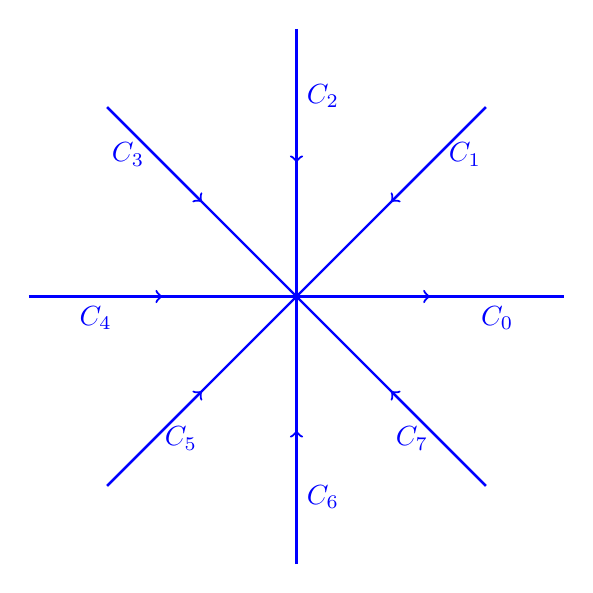
\begin{tikzpicture}[scale=0.85]
		\draw[blue, thick,->] (0,0) -- (2,0);
		\draw[blue, thick] (0,0) -- (4,0);
		\draw[blue, thick] (2,0) -- node[below] {$C_0$}(4,0);
		\draw[blue,thick,->] (0,4) -- node[right] {$C_2$}(0,2);
		\draw[blue, thick] (0,0) -- (0,4);
		\draw[blue,thick] (0,0) -- (2*99/70,2*99/70);
		\draw[blue,thick,->] (2*99/70,2*99/70) -- node[right] {$C_1$} (99/70,99/70);
		\draw[blue, thick] (0,0) -- (-4,0);
		\draw[blue, thick,->] (-4,0) -- node[below] {$C_4$} (-2,0);
		\draw[blue,thick,->] (0,-4) -- node[right] {$C_6$} (0,-2);
		\draw[blue,thick] (0,0) -- (0,-4);
		\draw[blue,thick] (0,0) -- (-2*99/70,-2*99/70);
		\draw[blue, thick,->] (-2*99/70,-2*99/70) -- node[right] {$C_5$} (-99/70,-99/70);
		\draw[blue,thick] (0,0) -- (-2*99/70,2*99/70);
		\draw[blue, thick,->] (-2*99/70,2*99/70) -- node[left] {$C_3$} (-99/70,99/70);
		\draw[blue, thick] (0,0) -- (2*99/70,-2*99/70);
		\draw[blue, thick,->] (2*99/70,-2*99/70) -- node[left] {$C_7$} (99/70,-99/70);
\end{tikzpicture}
\end{center}
\caption{This figure depicts the contours $C_0, \dots, C_{D-1}$ in the case $D=8$. The arrows denote the orientation of the contours. Note the outgoing orientation of $C_0$.}\label{contours}
\end{figure}

\begin{Proposition}\label{representation} Let $Q \in \mathscr{P}^\mathbb{C}$ be a polynomial, then $Q$ can written as
\begin{equation*}
Q(x) = {\rm e}^{V(x)} \frac{\rm d}{{\rm d}x}\big({\rm e}^{-V(x)} P(x) \big) = P^\prime(x) - V^\prime(x) P(x)
\end{equation*}
for some polynomial $P \in \mathscr{P}^\mathbb{C}$ if and only if the following integrals vanish:
\begin{align}\label{integrals}
\int_{\Gamma_k} Q(x){\rm e}^{-V(x)} {\rm d}x = 0,\qquad \forall k \in [\![ 1,D-1]\!]
\end{align}
\end{Proposition}
\begin{proof}
\enquote{Only if} is trivial since for $z \in C_k \setminus \{ 0 \}$, $z^{D} > 0$, hence $P(z){\rm e}^{-V(z)}$ is rapidly decreasing, hence
\begin{align*}
\int_{\Gamma_k} Q(x){\rm e}^{-V(x)} {\rm d}z = \int_{\Gamma_k} \frac{\rm d}{{\rm d}x}\big(P(x){\rm e}^{-V(x)}\big) {\rm d}x =0,\qquad \forall k \in [\![ 1,D-1]\!].
\end{align*}
For the converse claim, suppose the integrals \eqref{integrals} all vanish. Let us then divide $D$ into ${\deg Q+1}$ with remainder, so that $\deg Q+1 = D \ell + r$, where $\ell , r \in \mathbb{N}$ and $r \leq D-1$. We will construct a~certain polynomial $R$ as follows. If $\deg Q \leq D-2$, then $R:=Q$, so we may assume ${\deg Q \geq D-1}$. We can then factorise
\begin{equation*}
Q(x) = F_1 (x) V^\prime(x) + G_1(x),
\end{equation*}
where $F_1 \in \mathscr{P}^\mathbb{C}$ has degree $\deg Q - D+1$ and $G_1 \in \mathscr{P}^\mathbb{C}$ has degree at most $D-2$. We can then repeat the procedure,
\begin{gather*}
F_1^\prime(x) = F_2(x) V^\prime(x) + G_2(x), \qquad
F_2^\prime(x)= F_3(x) V^\prime(x) + G_3(x),\qquad \ldots, \\
F_{\ell-1}^\prime(x) = F_{\ell}(x) V^\prime(x) + G_{\ell}(x).
\end{gather*}
$F_j \in \mathscr{P}^\mathbb{C}$ has degree $\deg Q-Dj+1$ and $G_j \in \mathscr{P}^\mathbb{C}$ has degree at most $D-2$ for $j=1, \dots , \ell$. In particular $F_\ell$ has degree $r$ and so the process terminates at this stage. Let
\begin{equation*}
R(x) := G_1(x) + \dots + G_\ell(x) + F_\ell^\prime(x).
\end{equation*}
$R$ has degree at most $D-2$.

By repeated integration by parts, we see that
\begin{align*}
\int_{\Gamma_k} R(x) {\rm e}^{-V(x)} {\rm d}x = 0,\qquad \forall k \in [\![ 1,D-1]\!].
\end{align*}
We now claim that $R \equiv 0$. Consider the function
\begin{equation*}
C(z) \overset{\mathrm{def}}{=} {\rm e}^{V(z)}\int_z^{+\infty} R(x) {\rm e}^{-V(x)} {\rm d}x,
\end{equation*}
where the integration path is from $z \in \mathbb{C}$ to $0$ then from $0$ to $+\infty$. $C$ is clearly an entire function. We claim that as $|z| \to +\infty$, $C(z) \to 0$, uniformly in $\operatorname{arg} z $. Hence by Liouville's theorem $C \equiv 0$, and hence $R \equiv 0$.

From our assumptions,
\begin{align*}
\int_z^{+\infty} R(x) {\rm e}^{-V(x)} {\rm d}x = \int_z^{(+\infty) \cdot {\rm e}^{2\pi {\rm i} \frac{k}{D}}} R(x) {\rm e}^{-V(x)} {\rm d}x,\qquad \forall k \in [\![ 1,D-1]\!].
\end{align*}
Now introduce the function $\varphi(z) = \tilde{V}(z)^\frac{1}{D}$ \big(where $\tilde{V}(z) = \frac{1}{\gamma}V(z)$\big) which is holomorphic and injective so long as $|z|$ is sufficiently large, i.e., on a neighbourhood of (complex) infinity. Let us choose $k \in \{0, \dots, D-1\}$, so that
\[
 2\pi \frac{k-\frac{1}{2}}{D} \leq \arg \varphi(z) \leq 2\pi \frac{k+\frac{1}{2}}{D}
\]
 (this $k$ may not be unique but this does not matter). Let us also define $\arg$ so that there is no branch cut through this sector. Finally, let us choose the contour such that $\operatorname{Re} (V(z))$ is always non-decreasing along the contour. The existence of such a contour is proven in Lemma \ref{contour}. Integrating by parts, we find
\begin{align*}
\int_z^{(+\infty) \cdot {\rm e}^{2\pi {\rm i} \frac{k}{D}}} R(x) {\rm e}^{-V(x)} {\rm d}x = \frac{R(z)}{V^\prime(z)} {\rm e}^{-V(z)}+ \int_z^{(+\infty) \cdot {\rm e}^{2\pi {\rm i} \frac{k}{D}}} \frac{\rm d}{{\rm d}x}\left( \frac{R(x)}{V^\prime(x)} \right) {\rm e}^{-V(x)} {\rm d}x.
\end{align*}
\smash{$\frac{\rm d}{{\rm d}x}\big( \frac{R(x)}{V^\prime(x)} \big)$} is a rational function which scales like $x^{-2}$ and so for $|x|$ sufficiently large there is a~constant $\kappa>0$ such that \smash{$\big| \frac{\rm d}{{\rm d}x}\big( \frac{R(x)}{V^\prime(x)} \big)\big| \leq \kappa |x|^{-2}$}. Thus
\begin{equation*}
\bigg|{\rm e}^{V(z)} \int_z^{(+\infty) \cdot {\rm e}^{2\pi {\rm i} \frac{k}{D}}} R(x) {\rm e}^{-V(x)} {\rm d}x\bigg| \leq \frac{|R(z)|}{|V^\prime(z)|}+ \kappa\int_z^{(+\infty) \cdot {\rm e}^{2\pi {\rm i} \frac{k}{D}}}|x|^{-2} |{\rm d}x| \longrightarrow 0
\end{equation*}
as $z \to \infty$. This limit holds so long as $z$ is confined to the sector \smash{$ 2\pi \frac{k-\frac{1}{2}}{D} \leq \arg \varphi(z) \leq 2\pi \frac{k+\frac{1}{2}}{D}$}, however since there are only finitely many such sectors this limit thus holds uniformly in $\operatorname{arg} \varphi(z)$ (and so uniformly in $\operatorname{arg} z$). Thus $R \equiv 0$.

Finally, this shows that ${\rm e}^{V(z)} \int_z^{+\infty} Q(x) {\rm e}^{-V(x)} {\rm d}x$ is a polynomial, since if we factorise $Q$ and integrate by parts, we~find
\begin{equation*}
{\rm e}^{V(z)} \int_z^{+\infty} Q(x) {\rm e}^{-V(x)} {\rm d}x = F_1(z) + \dots + F_\ell(z),
\end{equation*}
which is a polynomial of degree $\deg Q - D + 1$.
\end{proof}

\begin{Lemma}\label{contour} Let $\tilde{V}(w) = \frac{1}{\gamma}V(w) = w^D + \mathcal{O}\big(w^{D-1}\big)$ and let \smash{$\varphi(w) := \tilde{V}(w)^\frac{1}{D}$}. There exists a~${\varrho > 0}$ sufficiently large such that $\varphi$ is analytic and injective on
\begin{equation*}
U_\varrho := \{ z \in \mathbb{C}\colon |z| > \varrho \}
\end{equation*}
and such that the following holds. For each $z \in U_\varrho$ such that
\smash{$\frac{2\pi ( k - \frac{1}{2})}{D} \leq \arg \varphi(z) \leq \frac{2\pi ( k + \frac{1}{2})}{D}$},
there is a of contour $\tau_z$ starting at $z$ and tending to \smash{$(+\infty) \cdot {\rm e}^{2\pi {\rm i} \frac{k}{D}}$} such that $\operatorname{Re} (V(w))$ is non-decreasing along the contour and $\int_{\tau_z}|x|^{-2} |{\rm d}x| \to 0$ as $|z| \to \infty$ uniformly in $\operatorname{arg} z$.
\end{Lemma}
\begin{proof}
Let
\begin{equation*}
\tilde{\tau} (s) =
\begin{cases}
 |\varphi(z)| \exp\big({\rm i} (1-s)\arg \varphi(z) + {\rm i}s\frac{2\pi k}{D} \big), & s \in [0,1] ,\\
 (|\varphi(z)|+s-1) \exp\big({\rm i} \frac{2\pi k}{D} \big), & s \in [1,+\infty). \\
\end{cases}
\end{equation*}
Then we choose our contour to be the preimage of $\tilde{\tau}$, that is $\tau= \varphi^{-1} \circ \tilde{\tau}$. From this, we see that $V(\tau(s)) = \gamma \tilde{\tau}(s)^D$. A short calculation then shows that for $s \in (0,1)$
\begin{equation*}
\frac{\rm d}{{\rm d}s} \operatorname{Re} (V(\tau(s))) = \gamma |\varphi(z)|^D D \left( \arg \varphi(z) - \frac{2\pi k}{D} \right) \sin\left( D (1-s) \left( \arg \varphi(z) - \frac{2\pi k}{D} \right) \right) \geq 0.
\end{equation*}
It is also easy to show for $s \in (1,+\infty)$, $\frac{\rm d}{{\rm d}s} \bigl(\operatorname{Re} \tilde{\tau}(s)^D\bigr) \geq 0$. Furthermore, $\varphi(w) = w (1+o(1))$ and~${\varphi^\prime(w) = 1+o(1)}$ uniformly on $U_\varrho$ as $\varrho \to +\infty$, and so $\int_\tau |x|^{-2} |{\rm d}x| \to 0$ as $|z| \to \infty$ uniformly in $\operatorname{arg} z$.
\end{proof}

A central result in the theory of orthogonal polynomials is that their zeros are simple and lie in the support of the weight function. The following proposition gives a partial extension of this to dual skew-orthogonal polynomials.
\begin{Proposition}
$\Psi_{2n}$ has at least $2n+1$ real zeros $($not counting multiplicity$)$, of which at least $2n+2-\frac{D}{2}$ must be simple. $\Psi_{2n+1}$ has at least $2n$ real zeros $($not counting multiplicity$)$, of which at least $2n - \frac{D}{2}$ must be simple.
\end{Proposition}
\begin{proof}
Let $ x_1, \dots, x_\ell$ be the collection of real zeros of $\Psi_{2n}$ with odd multiplicity, i.e., exactly those points on $\mathbb{R}$ at which $\Psi_{2n}$ changes sign, where we do not repeat according to multiplicity. Then $\Psi_{2n}(x)(x-x_1)\cdots (x-x_\ell)$ has the same sign everywhere and vanishes only on a finite set, hence
\begin{equation*}
\int_\mathbb{R} \Psi_{2n}(x)(x-x_1)\cdots (x-x_\ell) {\rm e}^{-2V(x)} {\rm d}x \neq 0 .
\end{equation*}
However, if $\ell \leq 2n$ then the above integral vanishes, thus $\ell \geq 2n+1$. Furthermore, it is easily seen that at least $2n+2-\frac{D}{2}$ of these must be simple. A similar argument works for $\Psi_{2n+1}$.
\end{proof}

We now arrive at a pair of Riemann--Hilbert problems, for the even and odd dual skew-orthogonal polynomials, respectively. In what follows, it is more convenient to ensure the uniqueness of the sequence by fixing the next-to-leading coefficient of~$\Psi_{2n+1}$ to be zero rather than~$P_{2n+1}$. We begin with the \enquote{even problem}, so called because the $(1,1)$ matrix element of the solution will turn out to be $\Psi_{2n}$.

\begin{rhp}[even problem]\label{evenrhp} Let $V$ be a real polynomial of even degree~${D \geq 2}$ and positive leading coefficient, $\Gamma_j$ be defined by \eqref{contour1} and \eqref{contour2}, and
\begin{equation}\label{gamma}
\Gamma = \bigcup_{j=1}^{D-1} \Gamma_j
\end{equation}
with the orientations of $\Gamma_j$ inherited by $\Gamma$ $($see, e.g., Figure {\rm\ref{contours}}$)$. We look for a $(D+1) \times (D+1)$ matrix valued function
\begin{equation*}
A_{n} \colon\ \mathbb{C}\setminus \Gamma \longrightarrow \mathcal{M}_{D+1}(\mathbb{C})
\end{equation*}
such that
\begin{enumerate}\itemsep=0pt
\item[$(1)$] $A_{n}$ is analytic on $\mathbb{C}\setminus \Gamma$ $($that is, its matrix elements are analytic on $\mathbb{C}\setminus \Gamma)$.
\item[$(2)$] $A_{n}$ has continuous boundary values up to $\Gamma \setminus \{ 0 \}$. That is, given $x \in \Gamma \setminus \{ 0 \}$, as $\mathbb{C}\setminus \Gamma \ni z \to x$ from either the $+$ $($left$)$ side or $-$ $($right$)$ side non-tangentially, the limit of $A_{n}(z)$ exists. These limits are denoted
\begin{align*}
A_{n}^+ \colon\ \Gamma \setminus \{ 0 \} \longrightarrow \mathcal{M}_{D+1}(\mathbb{C}),\qquad
A_{n}^- \colon\ \Gamma \setminus \{ 0 \} \longrightarrow \mathcal{M}_{D+1}(\mathbb{C})
\end{align*}
and are continuous functions. \enquote{Left} and \enquote{right} mean relative to the orientation of the contour. The boundary values are related by the \enquote{jump matrix}
\begin{align*}
A_{n}^{+}(x) = A_{n}^{-}(x)\left(
\begin{array}{ccccccccccccccccccc}
1 & {\rm e}^{-2V} \chi_\mathbb{R} & {\rm e}^{-V} \chi_{\Gamma_1} & \dots & {\rm e}^{-V} \chi_{\Gamma_{D-1}} \\
& 1 \\
& & 1 \\
& & & \ddots \\
& & & & 1 \\
\end{array} \right), \qquad x \in \Gamma \setminus \{ 0 \}.
\end{align*}
\item[$(3)$] $A_{n}$ is bounded in a neighbourhood of $0$.
\item[$(4)$] We have the asymptotic normalisation
\begin{align*}
A_{n}(z) = \big(\mathbb{I}+ \mathcal{O}\big(z^{-1}\big)\big) \left(\begin{matrix}
z^{2n+D-1} \\
& z^{-2n} \\
& & z^{-1} \\
& & & \ddots \\
& & & & z^{-1}
\end{matrix} \right),\qquad z \to \infty.
\end{align*}
\end{enumerate}
\end{rhp}
\begin{Lemma}\label{uniqueness} If a solution to Riemann--Hilbert Problem {\rm \ref{evenrhp}} exists, then it is unique.
\end{Lemma}
\begin{proof}
This method is standard but we repeat it for completeness. We note that the jump matrix has determinant $1$ so $\det A_{n}(z) $ has no jump across $\Gamma \setminus \{ 0 \}$ and takes continuous boundary values, so by Morera's theorem is analytic everywhere except possibly at $0$. However, the requirement of boundedness in a neighbourhood of $0$ implies that the singularity at $0$ is removable. Hence $z \mapsto \det A_{n}(z)$ is entire. Furthermore, we have the normalisation
$\det A_{n}(z) = 1 + \mathcal{O}\big(z^{-1}\big)$,
 as $z \to \infty$ and so $\det A_{n}(z) \equiv 1$.
Then let \smash{$\tilde{A}_{n}$} be another solution. Then the function \smash{$z \mapsto \tilde{A}_{n}(z) A_{n}^{-1}(z)$}
has no jump across $\Gamma \setminus \{0 \}$ and obtains continuous boundary values, so by Morera's theorem is analytic everywhere except possibly at $0$. Again by the requirement of boundedness of \smash{$\tilde{A}_n$} and $A_n$ in a neighbourhood of $0$ and that $\det A_n(z) \equiv 1$, we see that the singularity at $0$ is removable. Hence \smash{$z \mapsto \tilde{A}_{n}(z) A_{n}^{-1}(z)$} is actually entire. Finally, since
\begin{equation*}
\tilde{A}_{n}(z) A_{n}^{-1}(z) = \mathbb{I}+\mathcal{O}\big(z^{-1}\big),
\end{equation*}
we find that $\tilde{A}_{n}(z) A_{n}^{-1}(z) \equiv \mathbb{I}$.
\end{proof}

The jump condition implies that $(A_{n})_{11}$ is an entire function which scales like $z^{2n+D-1}$ as $z \to \infty$. It is therefore a monic polynomial of degree $2n+D-1$ by Liouville's theorem,
\begin{equation*}
(A_{n})_{11} := Q \in \mathscr{P}_{2n+D-1}^\mathbb{C}.
\end{equation*}
The Plemelj formula then implies that the first row of $A_{n}$ is
\begin{equation*}
\big( Q , C_{\mathbb{R}}\big({\rm e}^{-2V} Q\big) , C_{\Gamma_1}\big({\rm e}^{-V} Q\big) , \dots , C_{\Gamma_{D-1}}\big({\rm e}^{-V} Q\big)\big).
\end{equation*}
 From the asymptotic condition
 \begin{align*}
 C_{\Gamma_j}\big({\rm e}^{-V} Q\big)(z) = \mathcal{O}\big(z^{-2}\big),\qquad \forall j \in [\![ 1,D-1]\!],
 \end{align*}
we see, by Proposition \ref{representation}, that there exists a unique $P \in \mathscr{P}^\mathbb{C}$ of degree exactly $2n$ such that~${Q = {\rm e}^{V} \frac{\rm d}{{\rm d}x}\big(P {\rm e}^{-V}\big)}$. Finally, the normalisation
\begin{align*}
C_{\mathbb{R}}\big({\rm e}^{-2V} Q\big)(z) = \mathcal{O}\big(z^{-2n-1}\big) ,\qquad z \to \infty
\end{align*}
implies that $\langle \mathit{X}^k , P\rangle_4 =0 $ for $k \in [\![0, , 2n-1]\!]$, and so $P$ is skew-orthogonal. Thus $Q = \Psi_{2n}$.

For the second row, we see that $(A_{n})_{21} := \tilde{Q}$ is a polynomial of degree at most $2n+D-2$. Following the same procedure as above, we see that the second row is
\begin{equation*}
\big( \tilde{Q} , C_{\mathbb{R}}\big({\rm e}^{-2V} \tilde{Q}\big) , C_{\Gamma_1}\big({\rm e}^{-V} \tilde{Q}\big) , \dots , C_{\Gamma_{D-1}}\big({\rm e}^{-V} \tilde{Q}\big)
\big),
\end{equation*}
where now $\tilde{Q} = - \frac{2\pi {\rm i} \gamma D}{h_{n-2}} \Psi_{2n-2}$. For the remaining rows, we see that $(A_n)_{j+2,1} := R^{(j)}_n \in \mathscr{P}^{\mathbb{C}}_{2n+D-2}$ must be a polynomial of degree at most $2n+D-2$. To show there exists a unique solution to Riemann--Hilbert Problem~\ref{evenrhp}, let us introduce the following linear functionals:
\begin{align*}
\alpha_j \colon\ \mathscr{P}^{\mathbb{C}}_{2n+D-2} \longrightarrow \mathbb{C},\qquad
\beta_j \colon\ \mathscr{P}^{\mathbb{C}}_{2n+D-2} \longrightarrow \mathbb{C},
\end{align*}
where
\begin{align}
&\alpha_j(P) \overset{\mathrm{def}}{=} \int_\mathbb{R} {\rm e}^{-2V(x)} x^j P(x) {\rm d}x,\qquad j \in [\![ 0, 2n-1 ]\!],\label{alpha} \\
&\beta_j(P) \overset{\mathrm{def}}{=} -\frac{1}{2\pi {\rm i}} \int_{\Gamma_j} {\rm e}^{-V(x)} P(x) {\rm d}x,\qquad j \in [\![ 1, D-1]\!]. \label{beta}
\end{align}
\begin{Lemma}\label{linindep}The linear functionals $\alpha_0, \dots, \alpha_{2n-1}, \beta_1, \dots, \beta_{D-1}$ form a linearly independent set $\big($and thus span $\big(\mathscr{P}_{2n+D-2}^{\mathbb{C}}\big)^\ast\big)$.
\end{Lemma}

\begin{proof}
To show this, we need only show that
\begin{equation*}
\bigcap_{j=0}^{2n-1} \ker \alpha_j \cap \bigcap_{k=1}^{D-1} \ker \beta_k = 0.
\end{equation*}
Thus let \smash{$Q \in \mathscr{P}^\mathbb{C}_{2n+D-2}$} be such that $\alpha_0(Q) = \dots = \alpha_{2n-1}(Q)= \beta_1(Q) = \dots = \beta_{D-1}(Q)=0$. Thus by Proposition \ref{representation}, $Q = {\rm e}^V \frac{\rm d}{{\rm d}x}\big( P {\rm e}^{-V}\big)$ for some \smash{$P \in \mathscr{P}^\mathbb{C}_{2n-1}$}. Furthermore, $\smash{\big\langle \mathit{X}^0, P \big\rangle_4 =} \dots = \big\langle \mathit{X}^{2n-1}, P \big\rangle_4 = 0$. Hence $P$ is skew-orthogonal to all of \smash{$\mathscr{P}^\mathbb{C}_{2n-1}$}. Thus by the non-degeneracy of the inner product $\langle \cdot,\cdot \rangle_4$, $P \equiv 0$, and hence $Q \equiv 0$.
\end{proof}

Let \smash{$R^{(j)}_n \in \mathscr{P}^\mathbb{C}_{2n+D-2}$} be the unique polynomial such that
\smash{$
\alpha_0\big(R^{(j)}_n\big) = \dots = \alpha_{2n-1}\big(R^{(j)}_n\big) = 0
$}
and
\begin{align*}
\beta_k\big(R^{(j)}_n\big) = \delta_{kj},\qquad \forall k \in [\![ 1, D-1 ]\!].
\end{align*}
That such a polynomial exists and is unique follows from the linear independence of these functionals.

\begin{Theorem}
The unique solution of the \textit{even} Riemann--Hilbert Problem~{\rm \ref{evenrhp}} is
\begin{gather*}%\label{EvenSolution}
A_{n}
=\resizebox{.87\hsize}{!}{$\left(\begin{matrix}
\Psi_{2n} & C_\mathbb{R}\big({\rm e}^{-2V}\!\Psi_{2n}\big) & C_{\Gamma_1}\big({\rm e}^{-V}\!\Psi_{2n}\big) &\cdots & C_{\Gamma_{D-1}}\big({\rm e}^{-V}\!\Psi_{2n}\big) \\[1mm]
\!\!- \frac{2\pi {\rm i} \gamma D}{h_{n-1}}\Psi_{2n-2}\!\!\!\! & - \frac{2\pi {\rm i} \gamma D}{h_{n-1}} C_\mathbb{R}\big({\rm e}^{-2V}\!\Psi_{2n-2}\big)\!\!\!\! & - \frac{2\pi {\rm i} \gamma D}{h_{n-1}} C_{\Gamma_1}\big({\rm e}^{-V}\!\Psi_{2n-2}\big)\!\!\!\! & \cdots & \!\!\!\!\!- \frac{2\pi {\rm i} \gamma D}{h_{n-1}} C_{\Gamma_{D-1}}\big({\rm e}^{-V}\!\Psi_{2n-2}\big) \!\!\\[1mm]
R^{(1)}_n & C_\mathbb{R}\big({\rm e}^{-2V}\!R^{(1)}_n\big) & C_{\Gamma_1}\big({\rm e}^{-V}\!R^{(1)}_n\big) & \cdots & C_{\Gamma_{D-1}}\big({\rm e}^{-V}R^{(1)}_n\big) \\
\vdots \\
R^{(D-1)}_n & C_\mathbb{R}\big({\rm e}^{-2V}\!R^{(D-1)}_n \big) & C_{\Gamma_1}\big({\rm e}^{-V}\!R^{(D-1)}_n \big) & \cdots & C_{\Gamma_{D-1}}\big({\rm e}^{-V}R^{(D-1)}_n \big) \\
\end{matrix}\right)$}.
\end{gather*}
\end{Theorem}
